 \documentclass[10pt,a4paper]{ltjsarticle}       % LuaTeX を使う
\usepackage[luatex]{graphicx}             % LuaTeX 用, draft がついているときは図の代わりに同じ大きさの枠ができる
\usepackage{here}                               % 図表の位置を強制して出力
\usepackage{afterpage}                          % 残っている図を貼り付ける(\afterpage{\clearpage})
\usepackage[subrefformat=parens]{subcaption}    % サブキャプション(図1(a) とか)
\usepackage{setspace}                           % 行間制御
\usepackage{ulem}                               % 下線や取り消し線など
\usepackage{booktabs}                           % きれいな表(\toprule \midrule \bottomrule)
\usepackage{multirow}                           % 表で行結合
\usepackage{multicol}                           % 表で列結合
\usepackage{hhline}                             % 表で 2 重線
\usepackage[table]{xcolor}                      % カラー
\usepackage{tikz}                               % 図描画用
\usepackage[framemethod=tikz]{mdframed}         % 文章を囲むとき用
\usepackage[version=3]{mhchem}                  % 化学式
\usepackage{siunitx}                            % 単位
\usepackage{comment}                            % コメント
\setcounter{tocdepth}{3}                        % 目次に subsubsection まで表示
\usepackage{listings}
\lstset{
    frame=single,
    basicstyle=\small\ttfamily,
    tabsize=4,
    language=python,
    keywordstyle=\color{red},
    stringstyle=\color{blue}
}
% -----ヘッダ・フッタの設定-----
\usepackage{fancyhdr}
\usepackage{lastpage}
\pagestyle{fancy}
\lhead{}                                 % 左ヘッダ
\chead{}                                 % 中央ヘッダ
\rhead{}                                 % 右ヘッダ
\lfoot{}                                 % 左フッタ
\cfoot{\thepage~/~\pageref{LastPage}}    % 中央フッタ
\rfoot{}                                 % 右フッタ
\renewcommand{\headrulewidth}{0pt}       % ヘッダの罫線を消す
% -----余白の設定-----
% これをアンコメントするとページ番号が中央からずれるから今は使わない.
% \usepackage[left=19.05mm,right=19.05mm,top=25.40mm,bottom=25.40mm]{geometry}
% -----フォントの設定-----
% https://ja.osdn.net/projects/luatex-ja/wiki/LuaTeX-ja%E3%81%AE%E4%BD%BF%E3%81%84%E6%96%B9
% http://myfuturesightforpast.blogspot.jp/2013/12/tex-gyre.html など
\usepackage[no-math]{fontspec}
\usepackage{amsmath,amssymb}    % 高度な数式用
\usepackage{mathrsfs}           % 花文字用
% times ベース -> txfonts
% palatino ベース -> pxfonts
\usepackage{txfonts}
\usepackage{bm}                 % 斜体太字ベクトル
% Avant Garde -> TeX Gyre Adventor
% Bookman Old Style -> TeX Gyre Bonum
% Zapf Chancery -> TeX Gyre Chorus
% Courier -> TeX Gyre Cursor
% Helvetica -> TeX Gyre Heros
% Helvetica Narrow -> TeX Gyre Heros Cn
% Palatino -> TeX Gyre Pagella
% New Century Schoolbook -> TeX Gyre Schola
% Times -> TeX Gyre Termes
\setmainfont[Ligatures=TeX]{TeXGyreTermes}
\setsansfont[Ligatures=TeX]{TeXGyreHeros}
\setmonofont[Scale=MatchLowercase]{TeXGyreCursor}
\usepackage[match,deluxe,expert,bold]{luatexja-fontspec}
\setmainjfont[BoldFont=IPAexGothic]{IPAexMincho}
\setsansjfont{IPAexGothic}
\usepackage{luatexja-otf}
% -----PDF ハイパーリンク,ブックマーク,URL の設定-----
% オプション(\hypersetup{})は https://texwiki.texjp.org/?hyperref 参照
\usepackage{url}
% -----ソースコードの設定-----
% オプション(\lstset{})は http://tug.ctan.org/tex-archive/macros/latex/contrib/listings/listings.pdf 参照
% 使うときは
% \begin{lstlisting}[language=aaaa,caption=bbbb,label=List:cccc]
% hogehoge
% \end{lstlisting}
\usepackage{listings}
\lstset{%
  basicstyle=\ttfamily\small,%
  frame=single,%
  frameround=ffff,%
  numbers=left,%
  stepnumber=1,%
  numbersep=1\zw,%
  breaklines=true,%
  tabsize=4,%
  captionpos=t,%
  commentstyle=\itshape}
% -----図表等の reference の設定-----
% 表示文字列を日本語化
\renewcommand{\figurename}{図}
\renewcommand{\tablename}{表}
\renewcommand{\lstlistingname}{リスト}
\renewcommand{\abstractname}{概要}
% 図番号等を"<章番号>.<図番号>"
% lstlisting に関しては https://tex.stackexchange.com/questions/134418/numbering-of-listings 参照
\renewcommand{\thefigure}{\thesection.\arabic{figure}}
\renewcommand{\thetable}{\thesection.\arabic{table}}
\AtBeginDocument{\renewcommand{\thelstlisting}{\thesection.\arabic{lstlisting}}}
\renewcommand{\theequation}{\thesection.\arabic{equation}}
% 節が進むごとに図番号等をリセット
% http://d.hatena.ne.jp/gp98/20090919/1253367749 参照
\makeatletter
\@addtoreset{figure}{section}
\@addtoreset{table}{section}
\@addtoreset{lstlisting}{section}
\@addtoreset{equation}{section}
\makeatother
% \ref{} の簡単化
\newcommand*{\refSec}[1]{\ref{#1}~章}
\newcommand*{\refSsec}[1]{\ref{#1}~節}
\newcommand*{\refSssec}[1]{\ref{#1}~項}
\newcommand*{\refFig}[1]{\figurename~\ref{#1}}
\newcommand*{\refTab}[1]{\tablename~\ref{#1}}
\newcommand*{\refList}[1]{\lstlistingname~\ref{#1}}
\newcommand*{\refEq}[1]{式~(\ref{#1})}
% -----数式中便利な定義-----
% https://www.library.osaka-u.ac.jp/doc/TA_LaTeX2.pdf
% https://en.wikibooks.org/wiki/LaTeX/Mathematics など
\newcommand{\e}{\mathrm{e}}                     % ネイピア数
\newcommand{\imagi}{\mathrm{i}}                 % 虚数単位(i)
\newcommand{\imagj}{\mathrm{j}}                 % 虚数単位(j)
\newcommand{\vDel}{\varDelta}                   % デルタ大文字
\newcommand{\veps}{\varepsilon}                 % イプシロン小文字
\newcommand*{\paren}[1]{\left( #1 \right)}      % () を中身の大きさに合わせる
\newcommand*{\curly}[1]{\left\{ #1 \right\}}    % {} を中身の大きさに合わせる
\newcommand*{\bracket}[1]{\left[ #1 \right]}    % [] を中身の大きさに合わせる
\renewcommand{\Re}{\operatorname{Re}}           % 実部
\renewcommand{\Im}{\operatorname{Im}}           % 虚部
\newcommand*\sfrac[2]{{}^{#1}\!/_{#2}}          % xfrac パッケージの \sfrac{}{} の代わり
\renewcommand*\vec[1]{\mathbf{#1}}              % 矢印ベクトルは使わないので上書き.太字立体.
\newcommand{\argmax}{\mathop{\rm arg~max}\limits}
\newcommand{\argmin}{\mathop{\rm arg~min}\limits}

\title{知能システム論第3回課題}
\author{37186305\\航空宇宙工学専攻修士一年\\荒居秀尚}

\begin{document}
\maketitle

\section{ 宿題1}
\begin{equation}
\overline{X} - \overline{Y}\sim N \left( 
  \mu_{X} - \mu_Y, \frac{\sigma^2}{n_X}+\frac{\sigma^2}{n_Y}
\right)
\end{equation}
を示す。\\

\begin{align}
  E[\overline{X}- \overline{Y}] &= E\left[ \frac{1}{n_X} \sum_{i=1}^{n_X} X_i - \frac{1}{n_Y} \sum_{i=1}^{n_Y}Y_i\right] \\
   &= \frac{1}{n_X}\sum_{i=1}^{n_X}E[X_i] - \frac{1}{n_Y}\sum_{i=1}^{n_Y}E[Y_i] \\
   &= \mu_X - \mu_Y
\end{align}
\begin{align}
  V\left( \overline{X} - \overline{Y} \right) &= E\left[ \left(\overline{X} - \overline{Y}\right)^2 \right] - {\left\{ E\left[\overline{X} - \overline{Y}\right] \right\}}^2 \\
  &= E\left[\overline{X}^2\right] + E\left[\overline{Y}^2\right] - 2E\left[\overline{X}\overline{Y}\right] - {\left\{E\left[\overline{X}\right]\right\}}^2 - {\left\{E\left[\overline{Y}\right]\right\}}^2 + 2E\left[\overline{X}\right]E\left[\overline{Y}\right] \\
  &= E\left[\overline{X}^2\right] - {\left\{E\left[\overline{X}\right]\right\}}^2 + E\left[\overline{Y}^2\right] - {\left\{E\left[\overline{Y}\right]\right\}}^2 \\
  &= V\left(\overline{X}\right) + V\left(\overline{Y}\right) \\
  &= \frac{\sigma^2}{n_X}+\frac{\sigma^2}{n_Y}
\end{align}
正規分布の再生性から$\overline{X}-\overline{Y}$も正規分布に従うため、題意を得る。

\section{宿題2}
\subsection{A}
6が出る確率の上界は
\begin{equation}
P(|X-2.2|>2.8) <\frac{0.7}{2.8^2}=0.08928
\end{equation}
である。
\subsection{B}
1,2,3のいずれかが出る確率の下界は、4,5,6がでる確率の上界を1から引けば良い。
\begin{equation}
1-P(|X-2.2|>1.2) > 1-\frac{0.7}{1.2^2} = 0.5139
\end{equation}
である。
\section{宿題3}
\begin{lstlisting}
import numpy as np
import matplotlib.pyplot as plt


def calc_chi_square(size):
    X1 = np.random.normal(0.0, 1.0, (size, ))
    X2 = np.random.normal(0.0, 1.0, (size, ))
    return X1**2 + X2**2


def calc_avg(y):
    avgs = []
    for i in range(y.size):
        if i == 0:
            avgs.append(y[i])
        else:
            avgs.append((avgs[i - 1] + y[i]) / (i + 1))
    return np.array(avgs)


if __name__ == "__main__":
    y = calc_chi_square(10000)
    avgs = calc_avg(y)
    x = np.arange(1, 10001)

    plt.plot(x, avgs)
    plt.xlabel("$n$")
    plt.ylabel("$\overline{X}_{n}$")
    plt.grid(True)
    plt.savefig("chi_square_strong_row.eps")
\end{lstlisting}

\begin{figure}[htbp]
\begin{center}
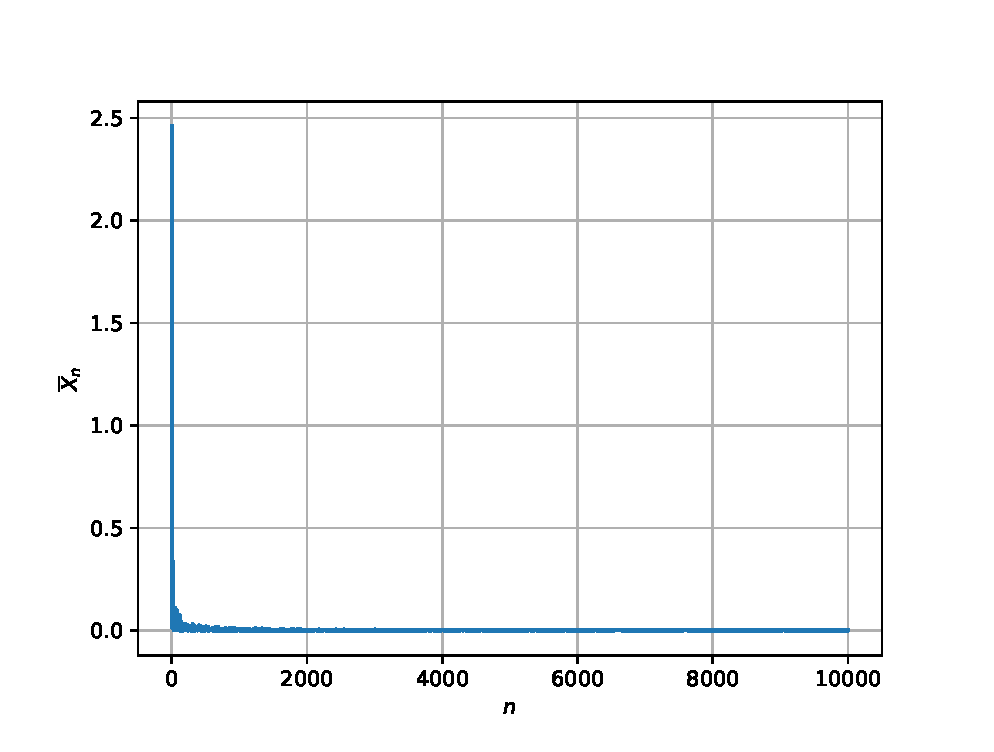
\includegraphics[clip, scale=0.7]{chi_square_strong_row.eps}
\caption{カイ二乗分布と大数の強法則}
\end{center}
\end{figure}
\clearpage
\begin{lstlisting}
import numpy as np
import matplotlib.pyplot as plt
import seaborn as sns


def chi_square(size):
    X1 = np.random.normal(0.0, 1.0, (size, ))
    X2 = np.random.normal(0.0, 1.0, (size, ))
    return X1**2 + X2**2


def chi_avg(chi):
    return chi.mean()


if __name__ == "__main__":
    color = ["r", "g", "b", "y", "k", "orange"]
    plt.figure()
    plt.ylabel("frequency")
    for i, c in enumerate(color):
        avg = [chi_avg(chi_square(i + 1)) for _ in range(10000)]
        sns.distplot(avg, color=c, label=f"n={i+1}")
    plt.legend()
    plt.savefig("chi_square_ultimate.eps")

\end{lstlisting}

\begin{figure}[htbp]
\begin{center}
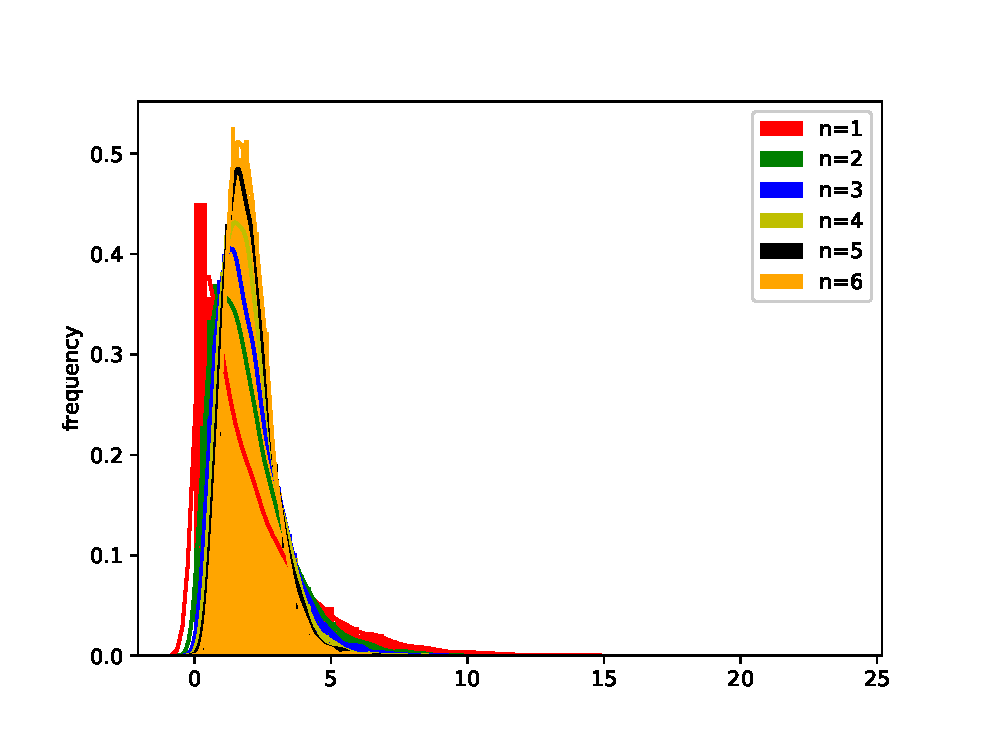
\includegraphics[clip, scale=0.7]{chi_square_ultimate.eps}
\caption{カイ二乗分布と中心極限定理}
\end{center}
\end{figure}
\clearpage
\begin{lstlisting}
import numpy as np
import matplotlib.pyplot as plt


def chi_square(size):
    X1 = np.random.normal(0.0, 1.0, (size, ))
    X2 = np.random.normal(0.0, 1.0, (size, ))
    return X1**2 + X2**2


def t_dist(size):
    X = np.random.normal(0.0, 1.0, (size, ))
    Y = chi_square(size)
    return np.divide(X, np.sqrt(Y / 2 + 1e-7))


def avg(t):
    avgs = []
    for i in range(t.size):
        if i == 0:
            avgs.append(t[i])
        else:
            avgs.append((avgs[i - 1] + t[i]) / (i + 1))
    return np.array(avgs)


if __name__ == "__main__":
    t = t_dist(10000)
    avgs = avg(t)
    x = np.arange(1, 10001)
    plt.plot(x, avgs)
    plt.xlabel("$n$")
    plt.ylabel("$\overline{X}_{n}$")
    plt.grid(True)
    plt.savefig("t_dist_strong_law.eps")

\end{lstlisting}

\begin{figure}[htbp]
\begin{center}
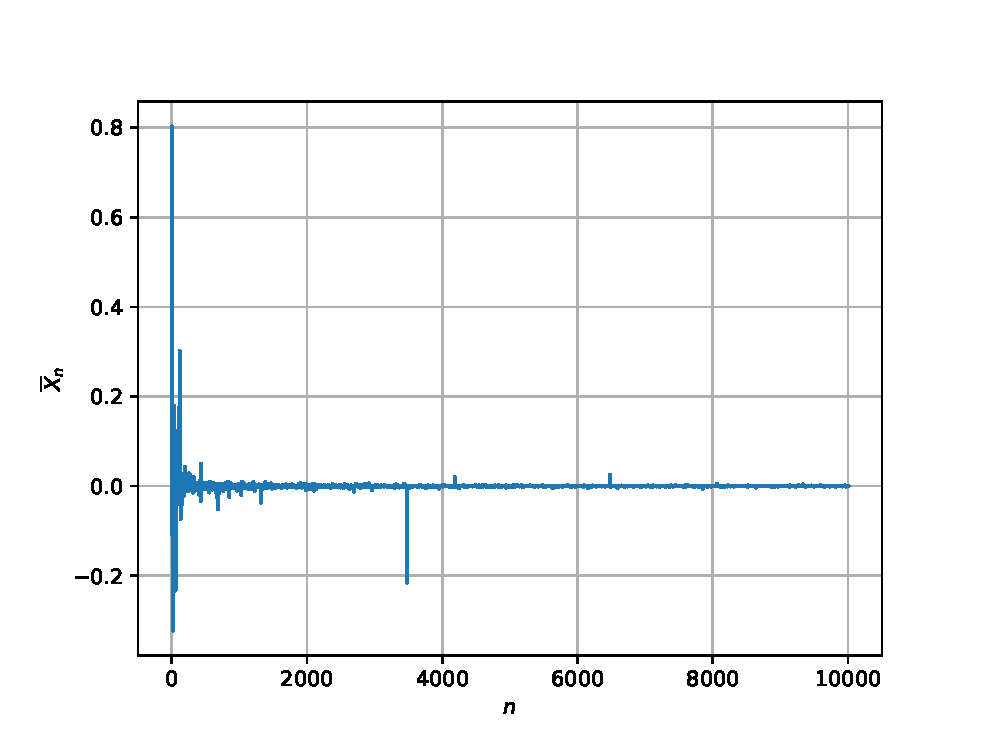
\includegraphics[clip, scale=0.7]{t_dist_strong_law.eps}
\caption{t分布と大数の強法則}
\end{center}
\end{figure}
\clearpage
\begin{lstlisting}
import numpy as np
import matplotlib.pyplot as plt
import seaborn as sns


def chi_square(size):
    X1 = np.random.normal(0.0, 1.0, (size, ))
    X2 = np.random.normal(0.0, 1.0, (size, ))
    return X1**2 + X2**2


def t_dist(size):
    X = np.random.normal(0.0, 1.0, (size, ))
    Y = chi_square(size)
    return np.divide(X, np.sqrt(Y / 2 + 1e-7))


def avg(t):
    return t.mean()


if __name__ == "__main__":
    color = ["r", "g", "b", "y", "k", "orange"]
    plt.figure()
    plt.ylabel("frequency")
    for i, c in enumerate(color):
        avgs = np.array([avg(t_dist(i + 1)) for _ in range(10000)])
        mean = avgs.mean()
        normalized = ((avgs - mean) / (1.0 / np.sqrt(i + 1)))
        sns.distplot(normalized, color=c, label=f"n={i+1}")
    plt.legend()
    plt.xlim(-10, 10)
    plt.savefig("t_dist_ultimate.eps")

\end{lstlisting}

\begin{figure}[htbp]
\begin{center}
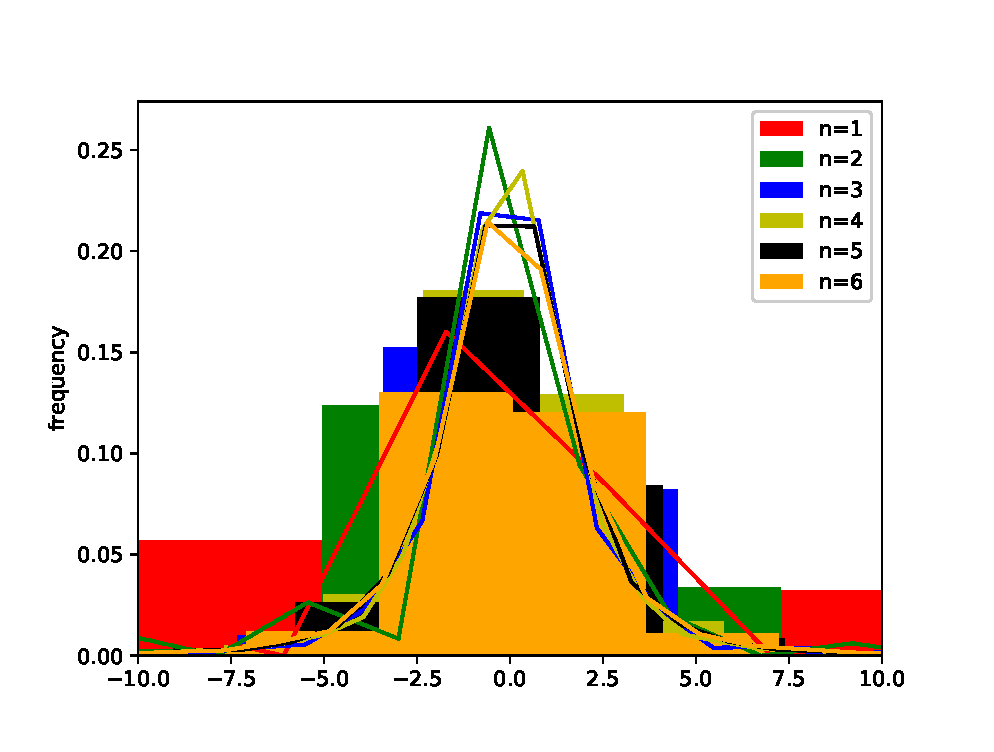
\includegraphics[clip, scale=0.7]{t_dist_ultimate.eps}
\caption{t分布と中心極限定理}
\end{center}
\end{figure}

\end{document}